\chapter{Marco teórico}

\section{Brazos robóticos industriales}

Antes de entrar en el tema principal de este documento, es importante conocer el antecedente o lo que se trata de mejorar, en nuestro caso, es imposible hablar de robots colaborativos sin primero abordar los brazos robóticos industriales.

Un brazo robótico es un manipulador, usualmente programable con funciones similares a las de un brazo humano. Los eslabones de este manipulador estan conectados por articulaciones que permiten el movimiento rotacional o translacional. \cite{ReviewRoboticArm} \cite{Schilling2001}

De acuerdo con \cite{Spong2005}, la mayoría de las aplicaciones en el campo de la robótica se centran en brazos robóticos industriales que operan en fabricas con entornos estructurados, es por esto su gran importancia.

La Federación Internacional de Robótica ha reportado un crecimiento promedio anual a partir del 2013 del 19\% en la demanda de brazos robóticos, siendo la industria automotríz la dominante, seguida por la industria eléctrica y electrónica. \cite{summary2019}


\subsection{Clasificación de los robots}

La clasificación de los brazos robóticos tiene dos grandes ramas, una de estas es por la fuente de su energía y la otra por la geometría de trabajo. 

La fuente de energía puede ser eléctrica o hidráulaca, la mayoría de los manipuladores hoy en día usan servomotores o motores a pasos de corriente continua \cite{Schilling2001}.

Dependiendo de la geometría de trabajo, los brazos robóticos  se dividen en: cartesianos, cilíndricos, esféricos, SCARA o articulados.


\section{Robótica colaborativa}

La robótica colaborativa surge como una rama de la robótica dispuesta a hacer más fácil el trabajo en lineas de producción, así como aliviar problemas en la espalda relacionados con tareas de ensamblado final en posiciones no ergonómicas \cite{cobot2018}\cite{cobotreview}.

Los robots colaborativos han sido desarrollados para trabajar de manera segura al lado de humanos, tomando en consideración la seguridad del operador, la del mismo robot y la correcta realización de la tarea a realizar.  Por esto, están equipados con medidas de seguridad para reconocer el ambiente en el que trabajan, tales como sistemas de evasión de obstáculos y detección de colisiones, implementadas a través de sensores o de mecanismos de compilación pasiva.

\paragraph{Escenarios de colaboración.} Es claro que no todas las aplicaciones donde se implemente un robot colaborativo requieren las mismas consideraciones, es por esto que existe una clasificación de acuerdo al grado de interacción con el operador y la dependencia entre éste y el robot colaborativo. Esos escenarios se mencionan a continuación y se ilustran en la figura \ref{fig:escenarioscolaborativos} \cite{Zaatari2019}.


\begin{itemize}
\itemsep0em
\item \textbf{Independiente.} Un operador y un robot colaborativo trabajan en distintas piezas de trabajo, cada uno con un proceso de manufactura individual. El elemento colaborativo es debido a la co-presencia en la misma área de trabajo.
\item \textbf{Simultanea.} Un operador y un robot colaborativo operan en procesos separados en la misma pieza de trabajo al mismo tiempo. No existe una dependencia de tarea entre ellos, sin embargo, el cobot debe estar conciente y respetar el espacio del operador.
\item \textbf{Secuencial.} Un operador y un cobot relizan un proceso de manufactura secuencial en la misma pieza de trabajo. Existe dependencia de tiempo entre ambos a lo largo del proceso.
\item \textbf{Soporte.} Un operador y un robot trabajan en el mismo proceso de manera interaciva. Existe una dependencia entre las acciones del robot y el operador, es decir, sin uno de ellos, la tarea no podría realizarse.
\end{itemize}

\begin{figure}
    \centering
    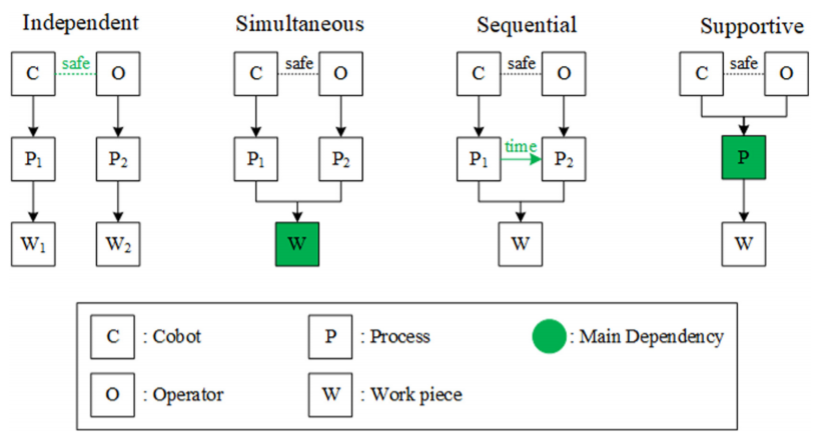
\includegraphics[scale=0.8]{./img/chapter2/escenarioscolaborativos.png}
    \caption{Escenarios colaborativos}
    \label{fig:escenarioscolaborativos}
\end{figure}

Con esto en mente, es fácil deducir que la mayoría de las investigaciones en el área de robótica colaborativa están encaminadas a estudiar o mejorar la detección de colisiones para salvaguardar la integridad de las personas que deberán trabajar junto a los cobots.

Incluso antes de que se acuñara el término cobots, ya había investigaciones encaminadas a la evasión de obstáculos \cite{Khatib1986}, dónde se plantea la solución a través de algoritmos de planeación de ruta.


En la mayoría de los robots colaborativos que existen en el mercado hoy en día se utilizan sensores de fuerza-torque en cada una de las articulaciones, sin embargo, los sensores montados en el robot colaborativo no son la única forma de proveer la seguridad necesaria, en \cite{Teke2018}, se aborda el uso de sensores de visión computacional a través del dispositivo Kinect V2 de Microsoft para modificar la trayectoria y así evadir obstáculos.

En \cite{Lu2005}, se concluye que es posible detectar colisiones utilizando sensores de fuerza-torque únicamente en la base y muñeca de un brazo robótico. Los sensores de fuerza-torque son sumamente caros, por esta razón existen investigaciones como \cite{Phan2018} donde se trabaja en desarrollar nuevos sensores de fuerza-torque con gran velocidad de respuesta y bajo costo.

De igual forma, se han desarrollado estudios sobre como es posible desarrollar robots colaborativos sin la necesidad de sensores de fuerza-torque.

En \cite{Matsumotoa}, se propone un método de detección de colisión basado en la ley de control no-lineal adaptativo, donde se utiliza la diferencia entre el torque obtenido realmente en contra del calculado basado en el modelo dinámico.

Por otra parte, en \cite{Chen2018} también se propone el desarollo de un algoritmo de detección de colisión basado en el modelo dinámico del robot, en este se utiliza la corriente suministrada al motor y la información que proporcionen los sensores de posición para medir discrepancias y detectar colisiones, lo que reduce el costo dedicado a sensores que requiere un robot colaborativo. En esta investigación se tratará de replicar esta metodología para lograr un algoritmo de detección de colisión.

Uno de los ejemplos más populares de robots colaborativos es la línea de robots UR creada por Universal Robots, quién ha vendido más de 39,000 unidades de estos cobots. Una imagen del mismo puede ser apreciada en la figura \ref{fig:ur5}.

\begin{figure}
    \centering
    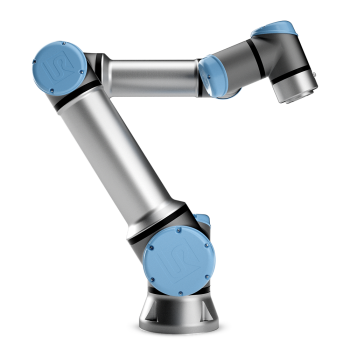
\includegraphics[scale=0.5]{./img/chapter2/ur5.png}
    \caption{Robot colaborativo UR5 de Universal Robots}
    \label{fig:ur5}
\end{figure}

\section{Sistemas de manufactura flexible}
\section{Ingeniería de sistemas basado en modelos}
